\documentclass[25pt,a0paper, portrait]{tikzposter}
\usepackage[utf8]{inputenc}
\usepackage{xcolor}
\usepackage{graphicx,mwe}
\usepackage{filecontents}
\usepackage{lipsum}
\usepackage{tikz}
\usepackage{multicol}
\usepackage{adjustbox}
\usepackage{blindtext}
\usepackage{comment}
\usepackage{amsmath}
\usepackage{booktabs}
\usepackage{graphicx}
\usetikzlibrary{positioning, arrows.meta, shapes.geometric, patterns, backgrounds}
\usepackage{csquotes}
\usepackage{xcolor}
\usepackage{array}

\makeatletter
\def\TP@titlegraphictotitledistance{-5.8cm}
\settitle{\centering\vbox{
		\raggedright\@titlegraphic
		\vspace*{-5.4cm}
		\centering
		\color{titlefgcolor}
		{\bfseries\Huge\sc\@title\par}
		\vspace*{0.6em}
		{\large\@author\par}
		\vspace*{0.3em}
		{\normalsize\@institute\par}
}}
\makeatother

\setlength{\columnsep}{1.5cm}

\title{Localization of a Mobile Robot}
\author{Srikanth Nanda: 7026002}
\institute{First examiner: Prof. Dr. Elmar Wings | Second examiner: Prof. Dr. Jonas Schwarz
	\quad\textbullet\quad Hochschule Emden/Leer}

\titlegraphic{
	\hbox to \linewidth{%
		
\includegraphics[height=3.4cm]{images/logo_hs_technik}%
		\hfill
	}
}

\usetheme{Desert}

\begin{document}
	
	\maketitle
	
	\begin{columns}
		
		%% ───────────────── LEFT COLUMN ─────────────────
		\column{0.5}
		{
			\colorlet{blocktitlebgcolor}{blue}
			
			\block{Problem Description}
			{
				Localization allows a mobile robot to estimate its position and orientation within an environment. GPS is unreliable indoors, so robots must rely on alternative sensing such as RF, inertial, or \textbf{vision-based} methods.\newline
				
				This project investigates indoor localization on a Mobile robot using \textbf{monocular ORB-SLAM} with a Leopard Imaging IMX219 8MP camera and a 128-core NVIDIA Jetson Nano. The system must estimate pose and build a map using only camera data under indoor conditions.\newline
				
				\textbf{Research Question:}
				\begin{quote}
					\textit{Can monocular ORB-SLAM be reliably deployed end-to-end on an embedded NVIDIA Jetson Nano platform for real-time indoor robot localization?}
				\end{quote}
				
				\textbf{Hardware Used:}
				\begin{itemize}
					\setlength{\itemsep}{2pt}
					\item \textbf{Mobile Robot} Jetbot Kit and Sparkfun Qwiic Parts
					\item \textbf{NVIDIA Jetson Nano} (128-core GPU)
					\item \textbf{Leopard Imaging IMX219} monocular camera
				\end{itemize}
				
				\textbf{Software Used:}
				\begin{itemize}
					\setlength{\itemsep}{2pt}
					\item \textbf{ROS Melodic} on JetPack 4.3, \textbf{Python} 2 \& 3, Keras, ORB-SLAM 2 \& 3 
				\end{itemize}
				
			}
			
			\block{Challenges}
			{
				\begin{itemize}
					\setlength{\itemsep}{4pt}
					
					\item \textbf{Scale Ambiguity}\\
					A single monocular camera cannot measure absolute depth; distances must be inferred via multi-view geometry.
					
					\item \textbf{Texture and Illumination}\\
					Feature-based methods rely on distinguishable texture. Low-texture surfaces, illumination changes, and occlusions reduce tracking reliability.
					
					\item \textbf{Dynamic Objects}\\
					Moving people or obstacles introduce outliers that can corrupt pose estimation if not rejected.
					
					\item \textbf{Embedded Compute Constraints}\\
					NVIDIA Jetson Nano has limited CPU/GPU resources, restricting the complexity of algorithms deployable in real time.
					
					\item \textbf{Integration Fragility}\\
					ORB-SLAM2/3, ROS Melodic (rosbuild), Python/Boost bindings, and JetPack 4.3 form a complex stack where small incompatibilities break end-to-end deployment.
				\end{itemize}
			}
			
			\block{Proposed Solution}
			{
				Each challenge is addressed through a specific methodological decision:
				
				\vspace{0.2cm}
				\begin{itemize}
					\setlength{\itemsep}{3pt}
					\item \textbf{Multi-View Geometry}\\
					Triangulation and bundle adjustment across multiple frames recover scale; loop closure corrects accumulated drift.
					
					\item \textbf{Robust Features (ORB)}\\
					ORB descriptors provide rotation, scale, and illumination invariance, improving matching in challenging indoor scenes.
					
					\item \textbf{Re-localization and Outlier Handling}\\
					Place recognition recovers from tracking failures; filtering reduces the impact of dynamic objects.
					
					\item \textbf{Embedded-Friendly SLAM}\\
					Keyframe-based SLAM and local map optimization balance accuracy and real-time performance on NVIDIA Jetson Nano.
					
					\item \textbf{Fallback Collision Avoidance}\\
					An ONNX-based collision-avoidance pipeline with ROS orchestration provides a practical navigation layer even when full monocular SLAM is not yet robust.
				\end{itemize}
				
				\vspace{0.1em}
				\begin{center}
					{\small
						\renewcommand{\arraystretch}{1.5}
						\begin{tabular}{lccp{12.7cm}}
							\toprule
							\textbf{Approach} & \textbf{Pose estimate} & \textbf{Map / collision output} & \textbf{Compatibility with the Mobile Robot} \\
							\midrule
							ORB-SLAM2 & Yes (visual SLAM) & Sparse feature map & NVIDIA Jetson Nano, ROS/bindings fragile \\
							CNN-based & No (implicit) & Collision probability only & fully onboard and reactive only \\
							CNN + ORB-SLAM2 & Yes & Pose + CNN collision fusion & integration blocked on NVIDIA Jetson Nano \\
							ORB-SLAM3 & Yes (visual/VI SLAM) & Rich multi-map support & Best on ROS2/desktop, off-board for Mobile Robot \\
							\bottomrule
					\end{tabular}}\\
					\vspace{0.3cm}
					{\small \textit{Table~1: Comparison of localization solutions proposed for the Mobile Robot platform.}}
				\end{center}
			

%				\vspace{0.1em}
				\textbf{Conclusion:}\\
				The thesis produced a well-structured onboard navigation stack and validated monocular ORB-SLAM on desktop datasets, but a fully stable end-to-end deployment on NVIDIA Jetson Nano under NVIDIA JetPack~4.3 and ROS Melodic was not yet achieved. The main limitation lies at the integration boundary between ORB-SLAM, ROS tooling, and Python/Boost bindings showing that hardware capability alone is not sufficient when ecosystem compatibility is fragile and violates NVIDIA policies.
				
			}
		}
		
		%% ───────────────── RIGHT COLUMN ─────────────────
		\column{0.5}
		{
			\colorlet{blocktitlebgcolor}{blue}
			
			\block{System Architecture \& Hardware}
			{
				\begin{center}
					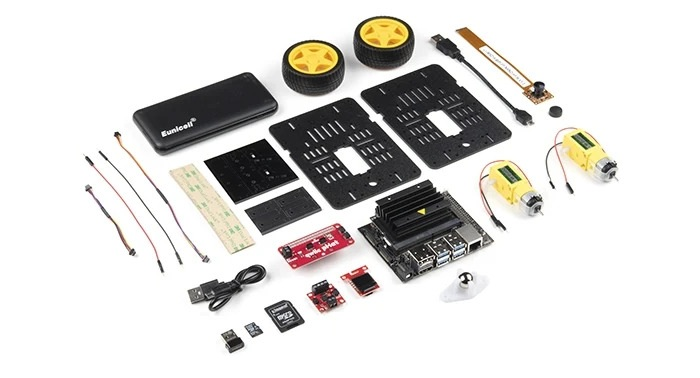
\includegraphics[width=0.85\linewidth, height=18cm, keepaspectratio]{images/MobileRobotParts.jpeg}\\
					\vspace{0.1cm}
					{\small \textit{Figure 1: Mobile robot kit components}}
				\end{center}
				
				\vspace{0.2cm}
				
				\begin{center}
					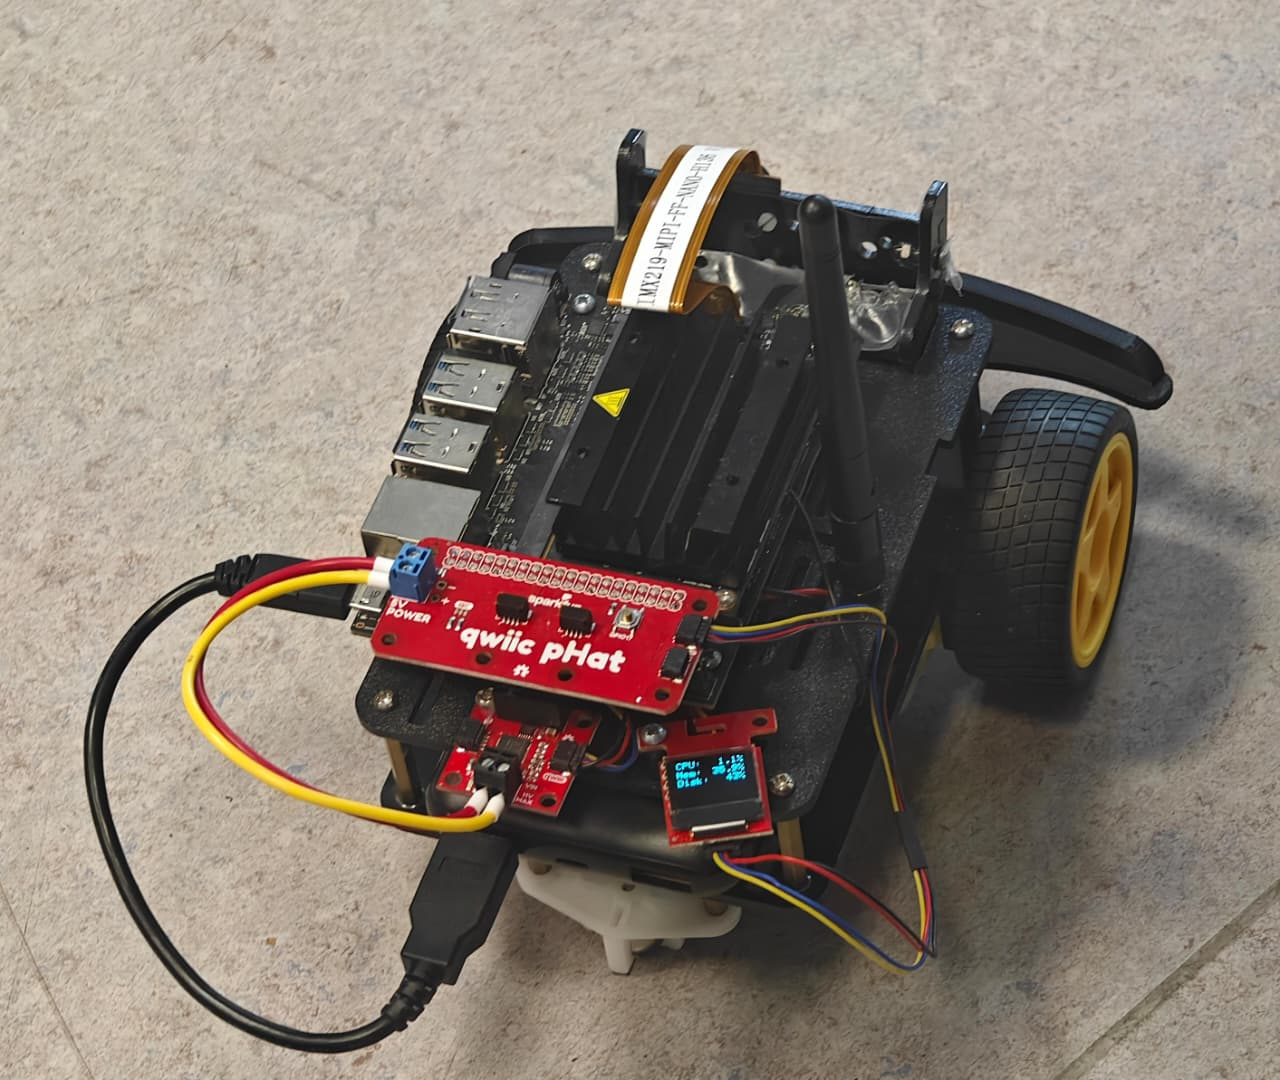
\includegraphics[width=0.90\linewidth, height=18cm, keepaspectratio]{images/Hardware.jpeg}\\
					\vspace{0.1cm}
					{\small \textit{Figure 2: Assembled Mobile Robot platform featuring NVIDIA Jetson Nano and Leopard Imaging IMX219 H136 8MP Camera and Sparkfun Qwiic parts.}}
				\end{center}
				
				\vspace{0.2cm}
				
				\begin{center}
					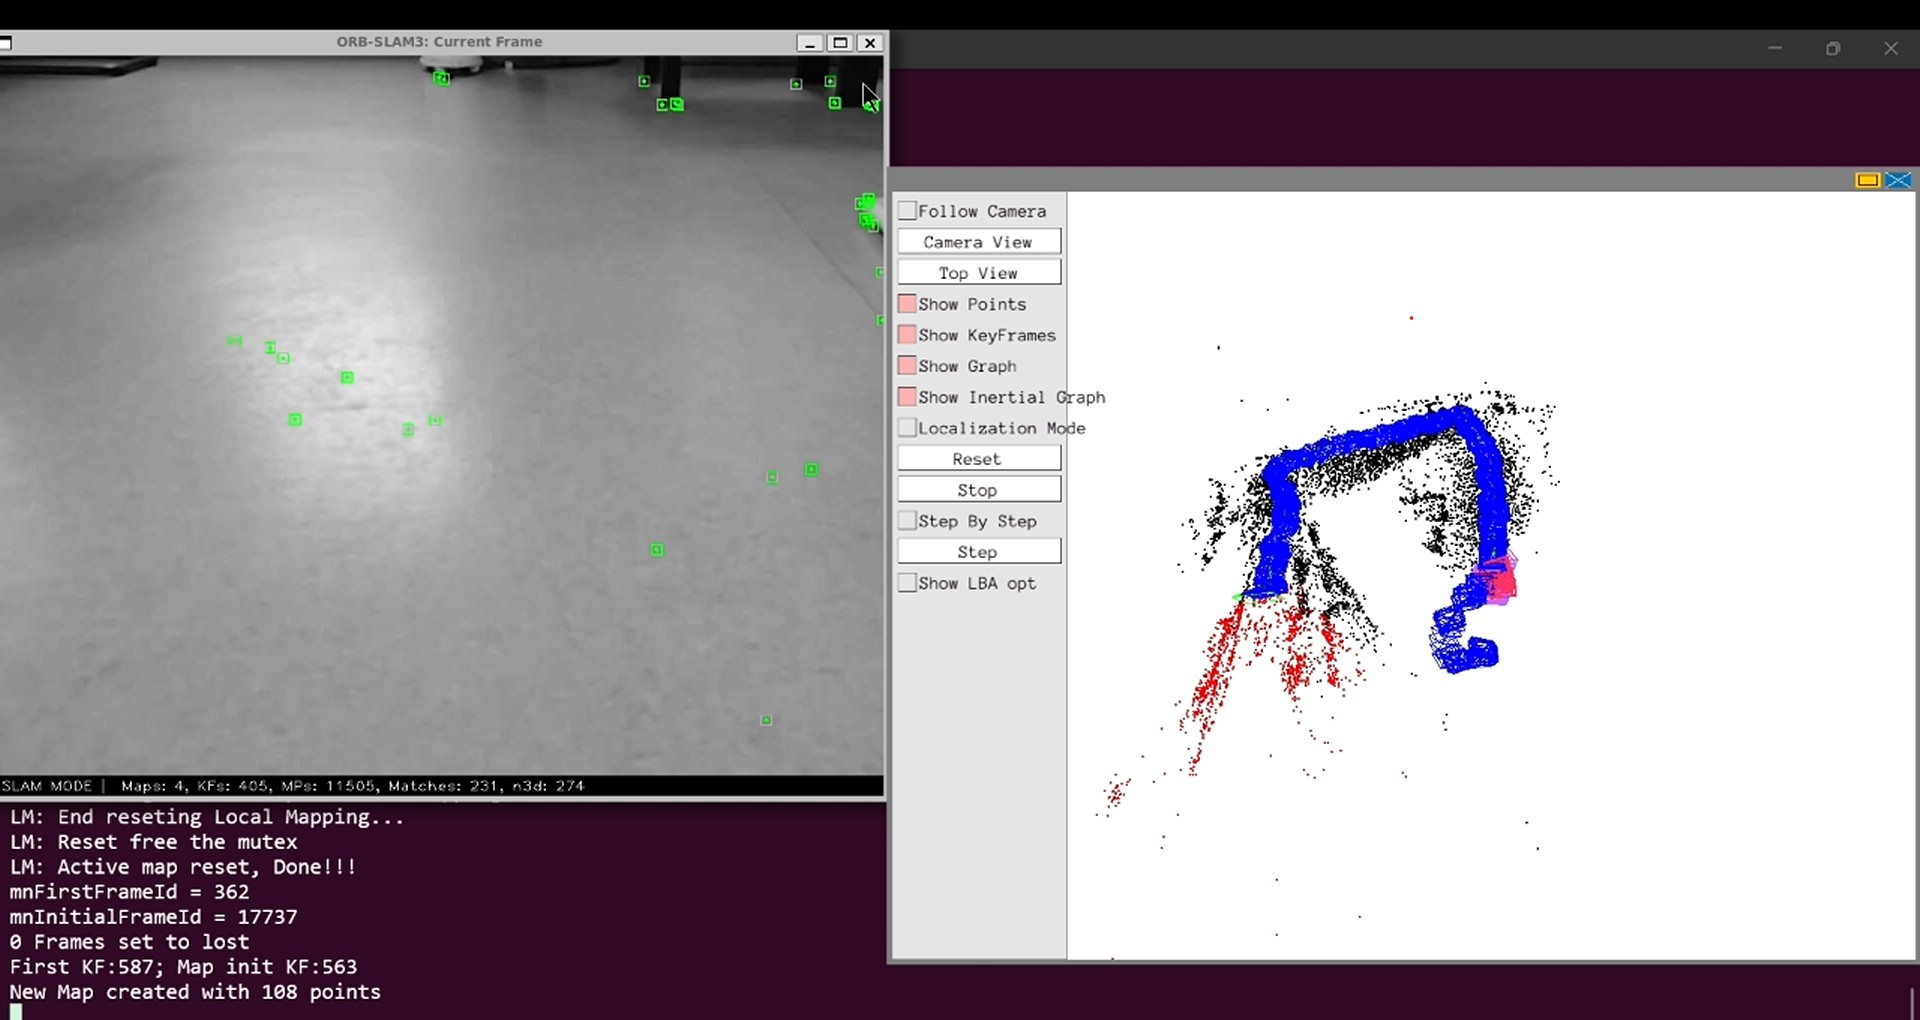
\includegraphics[width=0.95\linewidth, height=18cm, keepaspectratio]{images/Orbslam3.jpeg}\\
					\vspace{0.1cm}
					{\small \textit{Figure 3: ORB-SLAM3 running and tracking in the current frame and reconstructed map points.}}
				\end{center}
			}
			
			\block{Results}
			{
				\textbf{Positive Outcomes:}
				\begin{itemize}
					\setlength{\itemsep}{2pt}
					\item ORB-SLAM2 and ORB-SLAM3 built successfully as a standalone library
					\item Python navigation stack with occupancy grid and reactive decision node (slow/stop/recovery, heading stabilization)
					\item Functional ONNX collision-avoidance pipeline with ROS orchestration and telemetry logging
				\end{itemize}
				
				\vspace{0.2cm}
				
				\textbf{Integration Issues:}
				\begin{itemize}
					\setlength{\itemsep}{2pt}
					\item Python bindings for ORB-SLAM2 failed undefined symbol in the Boost/OpenCV converter layer
					\item \texttt{rosbuild}-based examples could not obtain compile flags under JetPack~4.3 / ROS Melodic
					\item Launch referenced a missing \texttt{orb\_slam2\_ros} package; only \texttt{/rosout} remained active
				\end{itemize}
				
				\vspace{0.1cm}
				
				\begin{center}
					\renewcommand{\arraystretch}{1.0}
					\begin{tabular}{lcc}
						\toprule
						\textbf{Component} & \textbf{Status} & \textbf{Notes} \\
						\midrule
						ORB-SLAM2 core lib & \textbf{Built} & Standalone \\
						Navigation stack   & \textbf{Working} & ONNX-based \\
						ROS integration    & \textbf{Working}         & rosbuild issue \\
						Python bindings    & Failed         & Boost symbol \\
						\bottomrule
					\end{tabular}
				\end{center}
				
				\vspace{0.4cm}
				
				ORB-SLAM3 successfully tracked features and reconstructed a sparse 3D map on the TUM benchmark dataset, confirming the algorithm's viability. However, porting this pipeline onto the NVIDIA Jetson Nano's ROS Melodic environment exposed integration failures that prevented a stable onboard deployment.
			}
		}
		
	\end{columns}
	
\end{document}